% Report: reinforcement learning for simplifying 3-manifold triangulations with Pachner moves.
% All numbers in tables/text come from ../results via ../scripts/make_tables.py (numbers.tex, tab_*.tex).
\documentclass[10pt,a4paper]{article}
\usepackage[a4paper,margin=1.85cm,top=1.6cm,bottom=1.7cm]{geometry}
\usepackage[T1]{fontenc}
\usepackage{mathptmx}
\usepackage[utf8]{inputenc}
\usepackage{microtype}
\usepackage{amsmath,amssymb}
\usepackage{graphicx,booktabs,xcolor,tikz}
\usepackage[hidelinks]{hyperref}
\usepackage[font=small,labelfont=bf,skip=3pt]{caption}
\usepackage{enumitem}
\usepackage{titlesec}
\titlespacing*{\section}{0pt}{7pt}{3pt}
\titlespacing*{\subsection}{0pt}{5pt}{2pt}
\titleformat{\section}{\large\bfseries}{\thesection}{0.6em}{}
\titleformat{\subsection}{\normalsize\bfseries}{\thesubsection}{0.5em}{}
\setlist{nosep,leftmargin=1.2em}
\setlength{\parindent}{0pt}\setlength{\parskip}{3.2pt}
\newcommand{\nReal}{750}
\newcommand{\nNTReal}{742}
\newcommand{\nTrivReal}{8}
\newcommand{\succrlReal}{56.5}
\newcommand{\succgreedyReal}{44.2}
\newcommand{\succgreedybalReal}{52.2}
\newcommand{\succgreedyplateauReal}{41.6}
\newcommand{\succrandomReal}{36.7}
\newcommand{\diffgreedyReal}{+12.3}
\newcommand{\logreedyReal}{+8.5}
\newcommand{\higreedyReal}{+16.0}
\newcommand{\pgreedyReal}{1.9e-11}
\newcommand{\diffgreedybalReal}{+4.3}
\newcommand{\logreedybalReal}{+0.8}
\newcommand{\higreedybalReal}{+8.1}
\newcommand{\pgreedybalReal}{0.017}
\newcommand{\diffgreedyplateauReal}{+14.8}
\newcommand{\logreedyplateauReal}{+11.2}
\newcommand{\higreedyplateauReal}{+18.5}
\newcommand{\pgreedyplateauReal}{1.6e-17}
\newcommand{\diffrandomReal}{+19.8}
\newcommand{\lorandomReal}{+15.3}
\newcommand{\hirandomReal}{+24.2}
\newcommand{\prandomReal}{1.2e-21}
\newcommand{\belowReal}{0}
\newcommand{\nSynth}{1000}
\newcommand{\nNTSynth}{994}
\newcommand{\nTrivSynth}{6}
\newcommand{\succrlSynth}{78.3}
\newcommand{\succgreedySynth}{75.2}
\newcommand{\succgreedybalSynth}{79.3}
\newcommand{\succgreedyplateauSynth}{76.1}
\newcommand{\succrandomSynth}{36.9}
\newcommand{\diffgreedySynth}{+3.1}
\newcommand{\logreedySynth}{+0.1}
\newcommand{\higreedySynth}{+6.0}
\newcommand{\pgreedySynth}{0.05}
\newcommand{\diffgreedybalSynth}{-1.0}
\newcommand{\logreedybalSynth}{-4.1}
\newcommand{\higreedybalSynth}{+2.0}
\newcommand{\pgreedybalSynth}{0.53}
\newcommand{\diffgreedyplateauSynth}{+2.2}
\newcommand{\logreedyplateauSynth}{-0.9}
\newcommand{\higreedyplateauSynth}{+5.3}
\newcommand{\pgreedyplateauSynth}{0.15}
\newcommand{\diffrandomSynth}{+41.3}
\newcommand{\lorandomSynth}{+37.7}
\newcommand{\hirandomSynth}{+44.9}
\newcommand{\prandomSynth}{2.2e-97}
\newcommand{\belowSynth}{0}
\newcommand{\trainList}{$4_1(5,1)$, $4_1(8,1)$, $4_1(9,1)$, $5_2(9,1)$, $5_2(11,1)$, $6_1(5,1)$, $6_1(9,1)$, $6_2(7,1)$, $6_3(5,1)$, $\mathrm{m006}(5,1)$, $\mathrm{m006}(7,1)$}
\newcommand{\gapMax}{2}
\newcommand{\gapMin}{0}
\newcommand{\nTrainInst}{11}
\newcommand{\nHeldInst}{5}
\newcommand{\restarts}{200}
\newcommand{\trSynth}{78}
\newcommand{\trSynthN}{97}
\newcommand{\trReal}{42}
\newcommand{\trRealN}{203}
\newcommand{\trRealNT}{38}
\newcommand{\trMaxStart}{27}
\newcommand{\zsN}{20}
\newcommand{\zsTarget}{9}
\newcommand{\chkOk}{90}
\newcommand{\chkOther}{0}
\newcommand{\cN}{15}
\newcommand{\cTargets}{4_1(5,1): 9, 5_2(7,1): 10}
\newcommand{\ftEpisodes}{200}
\newcommand{\ftBigReached}{7}
\newcommand{\ftBigN}{41}
\newcommand{\ftLastReached}{9}
\newcommand{\zsRLa}{0}
\newcommand{\zsMeanRLa}{25.9}
\newcommand{\zsSecsRLa}{1.1}
\newcommand{\zsGRa}{1}
\newcommand{\zsMeanGRa}{25.1}
\newcommand{\zsSecsGRa}{0.3}
\newcommand{\zsGBa}{1}
\newcommand{\zsMeanGBa}{20.8}
\newcommand{\zsSecsGBa}{0.4}
\newcommand{\zsRLb}{4}
\newcommand{\zsMeanRLb}{16.6}
\newcommand{\zsSecsRLb}{2.1}
\newcommand{\zsGRb}{11}
\newcommand{\zsMeanGRb}{10.9}
\newcommand{\zsSecsGRb}{0.6}
\newcommand{\zsGBb}{4}
\newcommand{\zsMeanGBb}{16.8}
\newcommand{\zsSecsGBb}{0.4}
\newcommand{\medKa}{3}
\newcommand{\medKb}{5}
\newcommand{\medKc}{9}
\newcommand{\gapWithinOne}{94}

% >>> replace with the real address of the code repository before submitting <<<
\newcommand{\repourl}{https://github.com/USERNAME/pachner-rl}
\newcommand{\eps}{\varepsilon}
\newcommand{\tet}{tetrahedra}

\title{\vspace{-0.9cm}\textbf{Teaching a computer to simplify 3-manifold triangulations\\ with reinforcement learning}\vspace{-0.2cm}}
\author{Lian de Souza Li \quad {\small IMECC/UNICAMP, Brazil}\\[-1pt] {\small Code: \url{\repourl}}}
\date{October 2026}

\begin{document}
\maketitle\vspace{-0.9cm}

\begin{abstract}\noindent
A closed 3-manifold has infinitely many triangulations, and finding a small one is a search problem on the graph of Pachner moves.
I train one shared reinforcement-learning (RL) agent, a Fitted-Q network that scores the legal 2-3, 3-2 and 4-4 moves, to shrink triangulations of
Dehn fillings of cusped census manifolds. Dehn fillings are an endless source of closed instances with a computable reference size (the best of many randomized SnapPy simplifications; not a proven minimum).
In a paired test in which every method starts from the same scrambled triangulation (\nNTReal{} non-trivial trials on five held-out fillings),
the agent reaches the reference size in \succrlReal\% of trials, against \succgreedyReal\% for a greedy baseline and \succgreedybalReal\% for a greedy baseline that picks move types evenly:
a clear gain over the first and a small one over the second. On scrambles of exactly 100 tetrahedra, far outside its training range, the agent does not beat greedy search.
All results are produced by the accompanying repository.
\end{abstract}

\section{Introduction and related work}
A closed 3-manifold $M$ can be assembled by gluing tetrahedra along their faces. The same manifold has infinitely many such \emph{triangulations}, of very different sizes, and
a smaller one makes almost every algorithm faster, from 3-sphere recognition \cite{thompson} to invariant computation (software such as Regina \cite{regina} and SnapPy \cite{snappy} simplify triangulations routinely).
Pachner's theorem \cite{pachner} says that any two triangulations of $M$ are joined by a finite sequence of local \emph{Pachner moves}, but not how long the sequence must be, nor how it should be chosen.
Greedy descent, which only applies size-reducing moves, gets stuck in local minima, and escaping them may require \emph{growing} the triangulation first.
For 3-sphere triangulations the necessary growth seems small: Burton's experiments on about $3\times10^7$ one-vertex triangulations with up to nine tetrahedra never needed more than two extra tetrahedra \cite{burton}; no such bound is known in general.

Machine learning has recently been applied to closely related combinatorial searches in low-dimensional topology.
Gukov et al.\ \cite{unknot} used RL to find Reidemeister-move sequences that unknot knot diagrams;
Applebaum et al.\ \cite{applebaum} used RL on diagrams with up to 200 crossings and determined the unknotting number of tens of thousands of knots;
Shehper et al.\ \cite{shehper} studied why rare, high-reward instances make Andrews--Curtis presentation problems hard for RL, and
Costantino, He, Heyes and Hirst \cite{chhh} analysed Pachner graphs of 3-manifold triangulations with network analysis and machine learning.
Learned heuristics for large move graphs also solve puzzles such as the Rubik's cube \cite{deepcubea}.
I ask the analogous question for triangulation simplification: \emph{can a single agent, trained across many manifolds, learn a useful policy for choosing Pachner moves?}
The answer found here is a measured ``partly'': a small advantage over strong hand-written heuristics on in-range instances, and none far outside the training range.

\section{Background}
\subsection{Triangulations and Pachner moves}
I work with one-vertex triangulations of closed orientable 3-manifolds, represented by SnapPy's \texttt{t3mlite} \texttt{Mcomplex}. Three Pachner moves are used (Figure~\ref{fig:moves}):
the \textbf{2-3} move replaces two tetrahedra sharing a face by three tetrahedra around a new edge ($+1$ tetrahedron, available across any interior face);
its inverse, the \textbf{3-2} move ($-1$), needs an edge of valence exactly 3; and the \textbf{4-4} move ($\pm0$) re-triangulates the four tetrahedra around a valence-4 edge.
The 1-4 and 4-1 moves are excluded because they change the number of vertices; for one-vertex triangulations the 2-3 and 3-2 moves alone already connect all triangulations of a manifold (Matveev, Piergallini; see \cite{matveev}).
The \emph{size} $n$ of a triangulation is its number of tetrahedra, and the task is to reach a small $n$ using the fewest, cheapest moves.

\begin{figure}[!t]
\centering
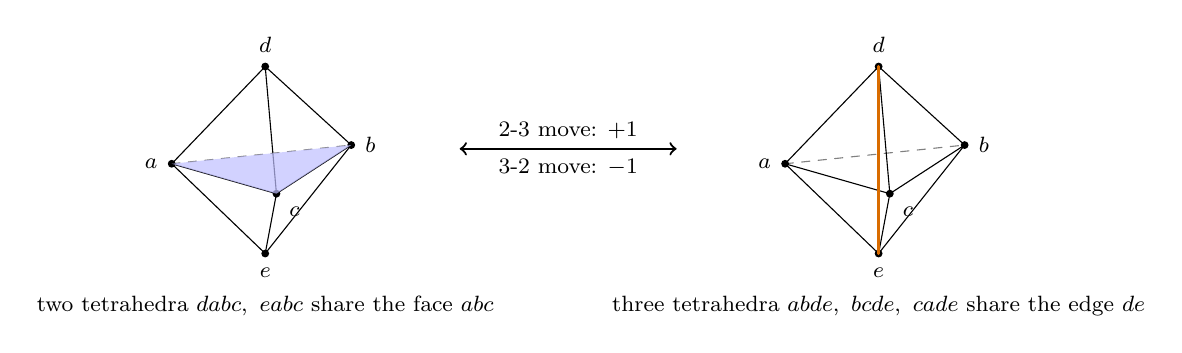
\begin{tikzpicture}[scale=0.95,line cap=round,every node/.style={font=\footnotesize}]
\tikzset{V/.style={circle,fill=black,inner sep=1pt},hid/.style={dashed,gray}}
\foreach \x/\lab in {0/{two tetrahedra $dabc,\ eabc$ share the face $abc$},8.2/{three tetrahedra $abde,\ bcde,\ cade$ share the edge $de$}}{
  \begin{scope}[xshift=\x cm]
  \coordinate (d) at (0,1.25); \coordinate (e) at (0,-1.25);
  \coordinate (a) at (-1.25,-0.05); \coordinate (b) at (1.15,0.2); \coordinate (c) at (0.15,-0.45);
  \draw[hid] (a)--(b); \draw (d)--(a)--(e)--(b)--(d); \draw (d)--(c)--(e); \draw (a)--(c)--(b);
  \node[V,label=above:$d$] at (d){}; \node[V,label=below:$e$] at (e){};
  \node[V,label=left:$a$] at (a){}; \node[V,label=right:$b$] at (b){}; \node[V,label=below right:$c$] at (c){};
  \node at (0,-1.95) {\lab};
  \end{scope}}
\fill[blue!25,opacity=.7] (-1.25,-0.05)--(1.15,0.2)--(0.15,-0.45)--cycle;
\draw[very thick,orange!85!black] (8.2,1.25)--(8.2,-1.25);
\draw[<->,thick] (2.6,0.15)--(5.5,0.15) node[midway,above]{2-3 move: $+1$} node[midway,below]{3-2 move: $-1$};
\end{tikzpicture}
\caption{The 2-3 / 3-2 move. The five vertices bound a bipyramid, split into two tetrahedra by the shared face $abc$ (blue) or into three by the new edge $de$ (orange, valence 3).}
\label{fig:moves}
\end{figure}

\paragraph{Why greedy fails.} Applying 3-2 moves while one exists always lowers $n$, but it stops when no valence-3 edge remains. 2-3 moves create valence-3 edges (the new edge) and 4-4 moves reshuffle valences at no cost, so good paths mix all three moves; which mix is the learning problem.

\subsection{Dehn fillings}
Let $M$ be a cusped manifold such as a knot complement, with torus boundary. Gluing a solid torus so that its meridian disc is attached along the slope $p\mu+q\lambda$ gives a closed manifold $M(p,q)$.
SnapPy's \texttt{filled\_triangulation()} returns a closed one-vertex triangulation of $M(p,q)$; I use these as start states. For example the figure-eight knot complement $4_1$ with slope $(5,1)$ gives a closed manifold with $H_1=\mathbb Z/5$ whose best-known triangulation has nine tetrahedra.

\subsection{Simplification as a Markov decision process}
\textbf{State.} Six hand-made features of the current triangulation: $n/n_0$, steps left over the budget, the fractions of edges with valence $\le3$, $=4$ and $\ge6$, and the edge count over $n_0$ ($n_0$ is the starting size).
\textbf{Actions.} Every legal 2-3, 3-2 and 4-4 move, each described by six features (type one-hot, change in $n$ over 3, mean and maximum valence of the edges involved).
\textbf{Reward.} For a successful move, $r=(n_t-n_{t+1})-0.02$; a failed move costs $-1$; reaching the target size gives $+5$ and ends the episode (the agent is not told the target in its state).
\textbf{Learner.} A Fitted-Q agent \cite{nfq}: an MLP (two hidden layers of 64 ReLU units, \texttt{scikit-learn}) maps (state, action) features to $Q$ and is regressed by Adam steps on minibatches from a replay buffer toward $r+\gamma\max_{a'}Q(s',a')$ with $\gamma=0.97$.
Because the network scores each legal move, a single network handles triangulations of any size and any number of legal moves.
Exploration is $\eps$-greedy with \emph{type-balanced} random moves (a move type is drawn first, then a move of that type), since a uniform draw over the move list would almost always pick a 2-3 move.
\textbf{Training loop.} At every step the agent picks a move ($\eps$-greedy), the environment applies it, the transition (features, reward, next legal moves) goes to a replay buffer (40\,000 transitions), and one minibatch of 256 transitions is regressed on the Fitted-Q targets. An episode ends at the target, at a step budget ($\le 50$ in training) or if $n>3n_0+10$.
Two details matter. First, the agent receives only generic features, never the target or the manifold, so one network serves every filling. Second, the next-state maximum ranges over \emph{all} legal moves, so the learned $Q$ can value a 2-3 move (a temporary $-1$ in reward) when it opens later 3-2 moves.

\section{Data}
\textbf{Closed instances from Dehn fillings.} Cusped census manifolds and coprime slopes $(p,q)$ give an unlimited supply of closed manifolds. Reference sizes are needed to know when a run succeeds, so for each filling I run \restarts{} randomized SnapPy simplifications
(\texttt{randomize()} followed by \texttt{simplify()}) on the filled manifold and keep the smallest triangulation found: the \emph{best-known} size, an upper bound for the true minimum. Over the \nTrainInst{} training and \nHeldInst{} held-out fillings, SnapPy's own start triangulation is 0--\gapMax{} tetrahedra above the best-known size, so the room to improve is small, which makes every tetrahedron count.
SnapPy's filled triangulations are random, so each filling's start triangulations are drawn once (a pool of up to 20) and stored by isomorphism signature in the repository; all evaluations reuse them.

\textbf{Training pool} (\nTrainInst{} fillings from six sources): \trainList. \textbf{Held-out test fillings} (unseen $(\text{knot},\text{slope})$ pairs):

\begin{center}\small
\begin{tabular}{@{}llccc@{}}\toprule
filling & SnapPy identification & $H_1$ & best-known $n$ & start sizes in pool\\\midrule
$4_1(7,2)$ & -- & Z/7 & 10 & 11--12 \\
$5_2(7,1)$ & $\mathrm{m015}(5,1)$ & Z/7 & 10 & 10--11 \\
$6_1(7,1)$ & -- & Z/7 & 16 & 16--17 \\
$6_3(7,1)$ & $\mathrm{s912}(7,1)$ & Z/7 & 17 & 17--19 \\
$\mathrm{m009}(5,1)$ & $\mathrm{m009}(5,1)$ & Z/2 + Z/4 & 11 & 11--11\\
\bottomrule\end{tabular}
\end{center}
\vspace{-4pt}
Fillings such as $5_2(7,1)$ and $6_3(7,1)$ are filled census manifolds (\texttt{m015}, \texttt{s912}) that also appear as training sources, so ``held-out'' means an unseen slope or knot, not an unrelated manifold family.

\begin{figure}[!t]
\centering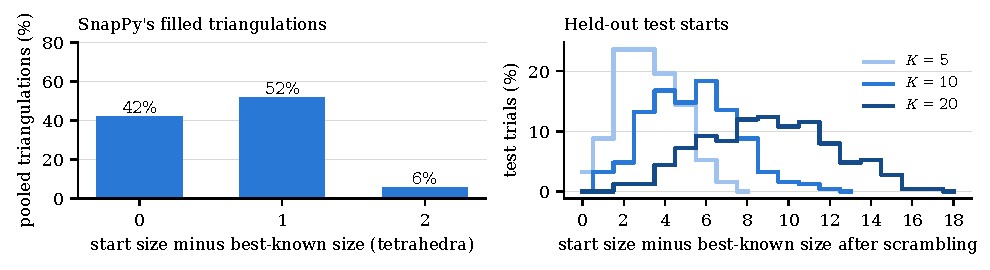
\includegraphics[width=\textwidth]{figs/fig_data.pdf}
\caption{\textbf{Left:} how far SnapPy's own filled triangulations are above the best-known size (all 16 fillings, pooled). \textbf{Right:} the same excess for the test starts after $K$ growth-biased scramble moves.}
\label{fig:data}
\end{figure}

\textbf{What the data look like.} SnapPy's filled triangulations are already within one tetrahedron of the best-known size for \gapWithinOne\% of the pool (Figure~\ref{fig:data}, left), so on its own a filled triangulation is a nearly trivial instance. The scrambles create the difficulty: after $K=5$, $10$, $20$ extra moves the median test start is \medKa, \medKb{} and \medKc{} tetrahedra above target, and the agent must undo that growth. Because the true minimum is unknown for real fillings, a success only means ``matched the best SnapPy found''; a run that beat it would count as a success too, and none did.

\textbf{Scrambles.} An episode starts from a pooled triangulation after $K$ extra growth-biased random moves (shrink bias $-0.6$): $K\in\{5,10,20\}$ at test time, $0$--$10$ during training. A start that is already at or below the target is counted as trivial and excluded from success rates.
To teach the agent the basic idea before the harder real data, training also uses \textbf{synthetic} episodes: census manifolds with known minimal size (\texttt{m003, m004, m015, m032, s912}; $n=2$--$6$) scrambled by 2--30 moves, with the exact minimum as target.
\textbf{Curriculum} (900 episodes, one shared agent): the synthetic share falls from 70\% to 30\%, scramble depth grows, and $\eps$ falls from 0.9 to 0.05. The agent sees neither the target nor whether an episode is real or synthetic.

\section{Results}
\subsection{Training}
Over the last 300 of 900 episodes the agent solved \trSynth\% of synthetic episodes ($n=\trSynthN$) and \trReal\% of real ones ($n=\trRealN$; \trRealNT\% excluding trivial starts); the largest training start had \trMaxStart{} tetrahedra (Figure~\ref{fig:tr}, left).
The synthetic curve declines as scrambles deepen and the real curve is roughly flat while its difficulty grows. These are training-pool numbers and say nothing about generalization.

\begin{figure}[!t]
\centering
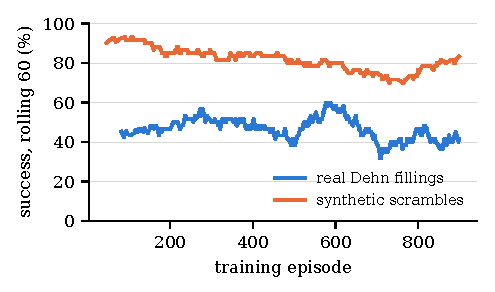
\includegraphics[width=0.485\textwidth]{figs/fig_training.pdf}\hfill
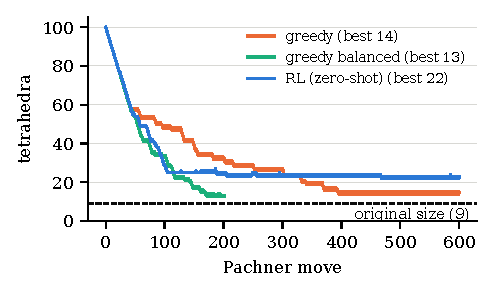
\includegraphics[width=0.485\textwidth]{figs/fig_traj100.pdf}
\caption{\textbf{Left:} training success (rolling mean over 60 episodes of each kind). \textbf{Right:} one 100-tetrahedron scramble of $4_1(5,1)$: identical start, 600-move budget; ``best'' is the smallest size reached.}
\label{fig:tr}
\end{figure}

\subsection{Held-out comparison with paired trials}
Every method starts from an \emph{identical} scrambled triangulation (same pooled start, same seeded scramble), so differences cannot come from easier starts; an earlier unpaired test with 10 trials per method had almost no power. Success means reaching the best-known size (real) or the known minimum (synthetic).
There are 50 seeds per (filling, $K$) and per (manifold, depth); uncertainty is a 95\% bootstrap interval over (filling, seed) clusters, and sign tests use trials where exactly one of two methods succeeds. Compared methods: the RL agent ($\eps=0.05$); \emph{greedy}, a 3-2 move if one exists and otherwise a random move from the whole list; \emph{balanced greedy}, the same with a type-balanced random fallback; greedy with a 4-4 fallback; and a biased random walk.

\begin{figure}[!t]
\centering
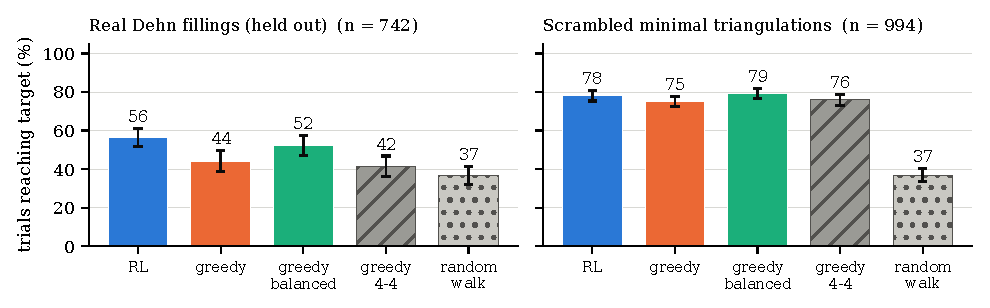
\includegraphics[width=\textwidth]{figs/fig_paired.pdf}
\caption{Share of non-trivial trials reaching the target (95\% cluster-bootstrap intervals). Left: five held-out fillings, $K\in\{5,10,20\}$, 50 seeds. Right: scrambles of five minimal census manifolds, depths 5--30, 50 seeds.}
\label{fig:paired}
\end{figure}

\begin{table}[!t]
\centering\small
\begin{tabular}{@{}lccr@{}}\toprule
 & success, \% [95\% CI] & RL minus method, points [95\% CI] & RL-only / other-only\\\midrule
\multicolumn{4}{@{}l}{\textit{Real held-out fillings} (\nNTReal{} non-trivial trials)}\\
RL agent & 56.5 [51.7, 61.2] & \multicolumn{2}{c}{--} \\
greedy (flat fallback) & 44.2 [38.9, 49.5] & $+12.3$ $[+8.5,+16.0]$ & 139/48 \\
greedy (balanced fallback) & 52.2 [47.0, 57.4] & $+4.3$ $[+0.8,+8.1]$ & 100/68 \\
greedy (4-4 fallback) & 41.6 [36.4, 46.8] & $+14.8$ $[+11.2,+18.5]$ & 143/33 \\
biased random walk & 36.7 [32.0, 41.6] & $+19.8$ $[+15.3,+24.2]$ & 198/51\\\midrule
\multicolumn{4}{@{}l}{\textit{Scrambled minimal manifolds} (\nNTSynth{} non-trivial trials)}\\
RL agent & 78.3 [75.4, 81.0] & \multicolumn{2}{c}{--} \\
greedy (flat fallback) & 75.2 [72.4, 77.9] & $+3.1$ $[+0.1,+6.0]$ & 133/102 \\
greedy (balanced fallback) & 79.3 [76.5, 81.9] & $-1.0$ $[-4.1,+2.0]$ & 96/106 \\
greedy (4-4 fallback) & 76.1 [73.1, 78.9] & $+2.2$ $[-0.9,+5.3]$ & 118/96 \\
biased random walk & 36.9 [33.6, 40.4] & $+41.3$ $[+37.7,+44.9]$ & 437/26\\
\bottomrule\end{tabular}
\caption{Paired comparison. ``RL-only / other-only'' counts trials in which exactly one of the two methods reached the target.}
\label{tab:paired}
\end{table}

\textbf{Aggregate.} On the real held-out fillings the agent reaches the target in \succrlReal\% of trials. This is clearly above the first greedy baseline (\diffgreedyReal{} points, CI [\logreedyReal, \higreedyReal]) and above the 4-4 and random-walk baselines, but only modestly above the balanced greedy
(\diffgreedybalReal{} points [\logreedybalReal, \higreedybalReal], sign test $p=\pgreedybalReal$, not corrected for four comparisons). An earlier run with freshly drawn start triangulations gave $+1.2$ [$-2.1$, $+4.6$] against the balanced greedy, so I trust the sign of this gap but not its size.
On synthetic scrambles the agent and balanced greedy are tied (\diffgreedybalSynth{} points [\logreedybalSynth, \higreedybalSynth]), and all three greedy variants beat the random walk by roughly 40 points.
The policies differ: by attempted moves the agent plays 45\% 3-2, 36\% 2-3 and 18\% 4-4 on real fillings, against 51/44/5 for flat greedy and 42/32/25 for balanced greedy. In none of the \nReal{} real and \nSynth{} synthetic trials did any method finish strictly below the target.

\begin{figure}[!t]
\centering
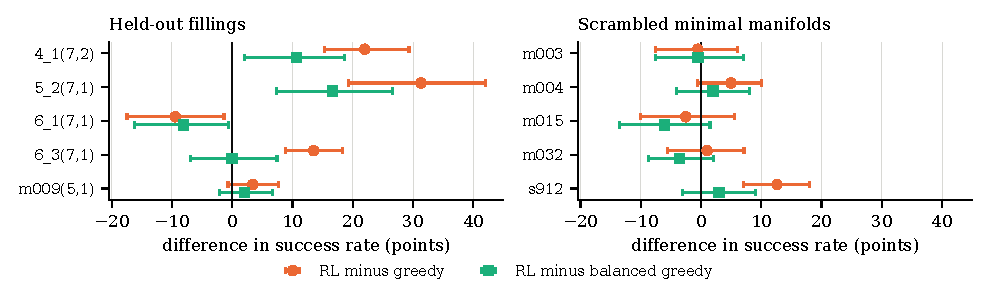
\includegraphics[width=\textwidth]{figs/fig_perfilling.pdf}
\caption{Difference in success rate, RL minus each greedy baseline, per instance (95\% bootstrap intervals over seeds). Positive values favour RL.}
\label{fig:forest}
\end{figure}

\textbf{Where the agent helps.} The aggregate hides large differences (Figure~\ref{fig:forest}). Against balanced greedy the agent is ahead on $5_2(7,1)$ and $4_1(7,2)$, level on $6_3(7,1)$ and $\mathrm{m009}(5,1)$, and \emph{behind} on $6_1(7,1)$; on synthetic scrambles it is level with balanced greedy on every manifold, and ahead of the first greedy only on \texttt{s912}.
I do not know why $6_1(7,1)$ is the exception; a plausible but untested explanation is that its start triangulations need a kind of 4-4 rearrangement that the six features cannot distinguish. Table~\ref{tab:byk} shows that the agent's lead on real fillings is largest for the longest scrambles ($K=20$: 62\% against 47\% and 52\%), while on synthetic scrambles all heuristics lose ground together as the depth grows and the agent's lead over balanced greedy is nil.

\begin{table}[!t]
\centering\small
\begin{tabular}{@{}lcccccc@{}}\toprule
setting & $n$ & RL & greedy & balanced & 4-4 greedy & random walk\\\midrule
fillings, $K$ 5 & 242 & 53 & 43 & 51 & 44 & 41 \\
fillings, $K$ 10 & 250 & 54 & 43 & 54 & 41 & 34 \\
fillings, $K$ 20 & 250 & 62 & 47 & 52 & 40 & 35 \\
minimal, depth 5 & 245 & 92 & 93 & 95 & 95 & 64 \\
minimal, depth 10 & 249 & 88 & 87 & 89 & 88 & 50 \\
minimal, depth 20 & 250 & 75 & 72 & 76 & 70 & 26 \\
minimal, depth 30 & 250 & 58 & 48 & 57 & 52 & 8\\
\bottomrule\end{tabular}
\caption{Success (\%) by scramble length, non-trivial trials.}
\label{tab:byk}
\end{table}

\subsection{Scaling to 100 tetrahedra}
To test scaling, I grow the base triangulation of $4_1(5,1)$ to exactly 100 tetrahedra with random 2-3 (and some 4-4) moves; the target is the original size, \zsTarget{} tetrahedra, with budgets of 180 or 600 moves. Every final triangulation that I checked (the first three scrambles of each method and configuration; \chkOk{} runs) still has the original homology and volume.
Applied unchanged, the agent---trained on starts of at most \trMaxStart{} tetrahedra---returns to the original size in \zsRLa/\zsN{} scrambles with 180 moves and \zsRLb/\zsN{} with 600, against \zsGRa/\zsN{} and \zsGRb/\zsN{} for greedy and \zsGBa/\zsN{} and \zsGBb/\zsN{} for balanced greedy. All methods fall quickly from 100 to about 25 tetrahedra (Figure~\ref{fig:tr}, right); the question is how often they get all the way back. The agent also costs more per run (\zsSecsRLa--\zsSecsRLb{} s against \zsSecsGRa--\zsSecsGRb{} s for greedy), as it scores every legal move with the network.

I then fine-tuned a copy of the agent for \ftEpisodes{} episodes on scrambles growing from 20 to 100 tetrahedra, with $\gamma=0.99$, a frozen target network re-synced every 150 updates and clipped targets (a first attempt with plain bootstrapping diverged), and compared all methods on fresh scrambles of $4_1(5,1)$ and of an unseen manifold, $5_2(7,1)$ (Table~\ref{tab:large}).
During the last 50 fine-tuning episodes (exploration on) the agent returned to the original size from \ftBigReached{} of \ftBigN{} starts with at least 90 tetrahedra, so it learned something on the training scrambles.

\begin{table}[!t]
\centering\small
\begin{tabular}{@{}lcccc@{}}\toprule
 & \multicolumn{2}{c}{$4_1(5,1)$, target 9} & \multicolumn{2}{c}{$5_2(7,1)$, target 10}\\
\cmidrule(lr){2-3}\cmidrule(lr){4-5}
 move budget & 180 & 600 & 180 & 600\\\midrule
RL zero-shot ($\varepsilon{=}0.05$) & 0 (24.2) & 2 (14.5) & 0 (25.7) & 2 (19.0) \\
RL fine-tuned ($\varepsilon{=}0.05$) & 1 (19.3) & 3 (16.6) & 1 (23.3) & 2 (19.3) \\
RL zero-shot ($\varepsilon{=}0$) & 1 (25.3) & 0 (19.9) & 0 (27.9) & 1 (23.5) \\
RL fine-tuned ($\varepsilon{=}0$) & 1 (20.5) & 2 (15.8) & 1 (23.4) & 1 (22.9) \\
greedy & 0 (24.5) & 8 (11.3) & 0 (28.7) & 5 (14.2) \\
greedy balanced & 3 (19.5) & 5 (15.8) & 1 (22.6) & 7 (17.2)\\
\bottomrule\end{tabular}
\caption{100-tetrahedron scrambles, \cN{} per cell: number returned to the original size (mean smallest size reached in brackets). $\eps$ is the exploration rate at test time.}
\label{tab:large}
\end{table}

Fine-tuning helps at the short budget (mean smallest size $4_1(5,1)$: 24.2 $\to$ 19.3), where the fine-tuned agent matches balanced greedy, but it does not help at 600 moves, where plain greedy is best on both manifolds (8/15 and 5/15 returns, against 3/15 and 2/15 for the fine-tuned agent). So the answer to ``does training at the target scale fix the scaling problem?'' is no, at least with 200 episodes and six-feature states. A plausible reason greedy does well here is that the scrambles are built from 2-3 moves, which 3-2 moves simply reverse; I did not test this.
With $\eps=0$ the agent can cycle between a 2-3 move and its inverse, which is why $\eps=0.05$ is used throughout.

\section{Conclusion and extensions}
\textbf{What the evidence says.} One shared agent, trained for 900 episodes on triangulations of at most \trMaxStart{} tetrahedra, chooses Pachner moves better than a naive greedy search and slightly better than a type-balanced greedy search on held-out fillings, with a filling-dependent margin. It does not reach 100 tetrahedra, even after fine-tuning. The main methodological lesson is that a baseline which merely balances move types removes most of the apparent RL gain, so paired comparisons against strong, cheap baselines are essential before claiming that RL has learned something.

\textbf{Reflections.} The evaluation design mattered more than the learning algorithm: the numbers that decide the story (a clear gain over one greedy rule, a small one over another, a loss at scale) only appeared once every method started from the same triangulation, once baselines were given a fair chance, and once the test was moved to unseen fillings and to a much larger size.
Dehn fillings were a convenient source of closed instances, but SnapPy's start triangulations are already close to the best-known size, so the headroom (0--\gapMax{} tetrahedra) is small, which caps what any method can show and makes differences of a few points fragile. A learned policy is also several times more expensive per run than a hand-written rule (3--4$\times$ at 100 tetrahedra), so it must clearly win to be worth using; at 100 tetrahedra it does not.

\textbf{Limits.} Reference sizes are best-known upper bounds, not proven minima, and the room to improve is only 0--\gapMax{} tetrahedra. There is one training run, so seed-to-seed variance of the agent is unmeasured; five held-out fillings, which share families with the training sources, give a narrow test; and six hand-made features discard most of the triangulation.

\textbf{Extensions.} (i) A graph neural network over the tetrahedron gluing graph would see the real combinatorics and could scale in size. (ii) More diverse training manifolds (larger fillings, other census families) and several training seeds would test generalization properly. (iii) Instances where growth is provably necessary, such as the sphere triangulations in Burton's study, would show whether RL finds genuinely non-greedy escapes rather than a better-tuned greedy rule.

\textbf{Reproducibility and use of LLMs.} Code, pinned environment, the trained checkpoint, the stored start triangulations and instructions are at \url{\repourl}; \texttt{scripts/reproduce.sh quick} takes about two minutes and \texttt{full} regenerates every table and figure here. Claude (Anthropic) assisted with code, analysis and drafting; I ran and checked the code, and every number above is generated by the repository scripts from stored results.

\clearpage
\begin{thebibliography}{99}\small\setlength{\itemsep}{0pt}
\bibitem{pachner} U. Pachner, P.L. homeomorphic manifolds are equivalent by elementary shellings, \emph{European J.\ Combin.} 12 (1991) 129--145.
\bibitem{thompson} A. Thompson, Thin position and the recognition problem for $S^3$, \emph{Math.\ Res.\ Lett.} 1 (1994) 613--630.
\bibitem{burton} B. A. Burton, The Pachner graph and the simplification of 3-sphere triangulations, \emph{Proc.\ SoCG} 2011, 153--162 (arXiv:1011.4169).
\bibitem{matveev} S. Matveev, \emph{Algorithmic Topology and Classification of 3-Manifolds}, 2nd ed., Springer, 2007.
\bibitem{regina} B. A. Burton, R. Budney, W. Pettersson et al., Regina: software for low-dimensional topology, \url{https://regina-normal.github.io}.
\bibitem{snappy} M. Culler, N. M. Dunfield, M. Goerner, J. R. Weeks, SnapPy, a computer program for studying the geometry and topology of 3-manifolds, \url{https://snappy.computop.org}.
\bibitem{unknot} S. Gukov, J. Halverson, F. Ruehle, P. Sułkowski, Learning to unknot, \emph{Mach.\ Learn.: Sci.\ Technol.} 2 (2021) 025035.
\bibitem{applebaum} T. Applebaum, S. Blackwell, A. Davies, T. Edlich, A. Juh\'asz, M. Lackenby, N. Tomašev, D. Zheng, The unknotting number, hard unknot diagrams, and reinforcement learning, arXiv:2409.09032 (2024).
\bibitem{shehper} A. Shehper et al., What makes math problems hard for reinforcement learning: a case study, arXiv:2408.15332 (2024).
\bibitem{chhh} F. Costantino, Y.-H. He, E. Heyes, E. Hirst, Learning 3-manifold triangulations, \emph{J.\ Phys.\ A} 58 (2025) 095201 (arXiv:2405.09610).
\bibitem{deepcubea} F. Agostinelli, S. McAleer, A. Shmakov, P. Baldi, Solving the Rubik's cube with deep reinforcement learning and search, \emph{Nat.\ Mach.\ Intell.} 1 (2019) 356--363.
\bibitem{nfq} M. Riedmiller, Neural fitted Q iteration, \emph{ECML 2005}, LNCS 3720, 317--328.
\end{thebibliography}

\appendix
\section{Details}\label{app:inst}
\textbf{Hyperparameters.} MLP $(12\to64\to64\to1)$, ReLU, Adam (lr $10^{-3}$), $\gamma=0.97$ ($0.99$ for 100-tet fine-tuning), minibatch 256, replay 40\,000, step cost $0.02$, failed move $-1$, success bonus $+5$, early stop at $n>3n_0+10$, training step budget $\min(50,\,3\cdot\text{extra}+20)$ (real) or $\min(45,\,3\cdot\text{depth}+10)$ (synthetic); exploration $\eps$ decays linearly from 0.9 to 0.05 over the first 70\% of the 900 episodes. 100-tet fine-tuning: scramble sizes 20--30 up to 100 over the first 60\% of episodes, budgets 180/600, target network re-synced every 150 updates, targets clipped to $[-10,100]$.

\textbf{Per-filling success (\%)} on the real held-out fillings, non-trivial trials ($n$ = trials):
\begin{center}\small
\begin{tabular}{@{}lcccccc@{}}\toprule
filling & $n$ & RL & greedy & balanced & 4-4 greedy & random walk\\\midrule
$4_1(7,2)$ & 150 & 35 & 13 & 25 & 13 & 17 \\
$5_2(7,1)$ & 150 & 44 & 13 & 27 & 11 & 12 \\
$6_1(7,1)$ & 148 & 70 & 80 & 78 & 75 & 61 \\
$6_3(7,1)$ & 148 & 36 & 23 & 36 & 22 & 20 \\
$\mathrm{m009}(5,1)$ & 146 & 97 & 94 & 95 & 88 & 74\\
\bottomrule\end{tabular}
\end{center}
\end{document}
